\chapter{Further Notes}








\section{Computation} \label{sec:notes_computation}


\subsection{Hardware and software} \label{sec:notes_hardware}

The hardware used for computation was an \emph{Intel Core i7-4790} CPU at 3.60\,GHz, with 32\,GB of RAM. The software used was R 3.5.1 \cite{r_rsoftware}, along with several R packages:
%
%
\begin{itemize}
	\item \textbf{igraph} \cite{r_igraph} for plotting networks
	\item \textbf{LICORS} \cite{r_LICORS} for an implementation of $k$-means++
	\item \textbf{mclust} \cite{r_mclust} for an implementation of ARI
	\item \textbf{rnaturalearth} \cite{r_rnaturalearth} for world territory boundary data
	\item \textbf{RSpectra} \cite{r_RSpectra} for eigendecomposition of sparse matrices
	\item \textbf{USAboundaries} \cite{r_USAboundaries} for US county and state boundary data
\end{itemize}






\subsection{Timings for MAM computations} \label{sec:notes_timing}

We record timings (in seconds) for the MAM formulae given in Table~\ref{tab:motif_adj_mat_table}. We test on DSBMs (Section~\ref{sec:motif_dsbms}) with $k=1$, and vary the graph size $n$ and sparsity parameter $p$.

\vspace*{0.3cm}
\begin{table}[H]
\centering
\renewcommand{\arraystretch}{1.5}
\setlength\tabcolsep{0.2em}
\scriptsize
	\begin{tabular}{ |c|c|c|c|c|c|c|c|c|c|c|c|c|c|c|c|c|c| }
		\hline	
		\input{../../results/timing/timing_n_100.txt}
	\end{tabular}
	\caption{Timings for MAM computation with $n=100$}
	\label{tab:timing_n_100}
\end{table}



\begin{table}[H]
\centering
\renewcommand{\arraystretch}{1.5}
\setlength\tabcolsep{0.2em}
\scriptsize
	\begin{tabular}{ |c|c|c|c|c|c|c|c|c|c|c|c|c|c|c|c|c|c| }
		\hline	
		\input{../../results/timing/timing_n_1000.txt}
	\end{tabular}
	\caption{Timings for MAM computation with $n=1000$}
	\label{tab:timing_n_1000}
\end{table}


\begin{table}[H]
\centering
\renewcommand{\arraystretch}{1.5}
\setlength\tabcolsep{0.2em}
\scriptsize
	\begin{tabular}{ |c|c|c|c|c|c|c|c|c|c|c|c|c|c|c|c|c|c| }
		\hline	
		\input{../../results/timing/timing_n_10000.txt}
	\end{tabular}
	\caption{Timings for MAM computation with $n=10 \, 000$}
	\label{tab:timing_n_10000}
\end{table}




\section{Data preprocessing} \label{sec:notes_preprocessing}

All real networks were preprocessed by restriction to their largest connected component. The Unicode Languages network in Section~\ref{sec:bipartite_languages} was also preprocessed to remove territories with under one million inhabitants and languages with under one million speakers. Vertex and edge counts of all networks are stated \emph{after} this preprocessing.





\section{US map} \label{sec:notes_us_map}
%
\vspace*{-0.8cm}
\begin{figure}[H]
	\centering
	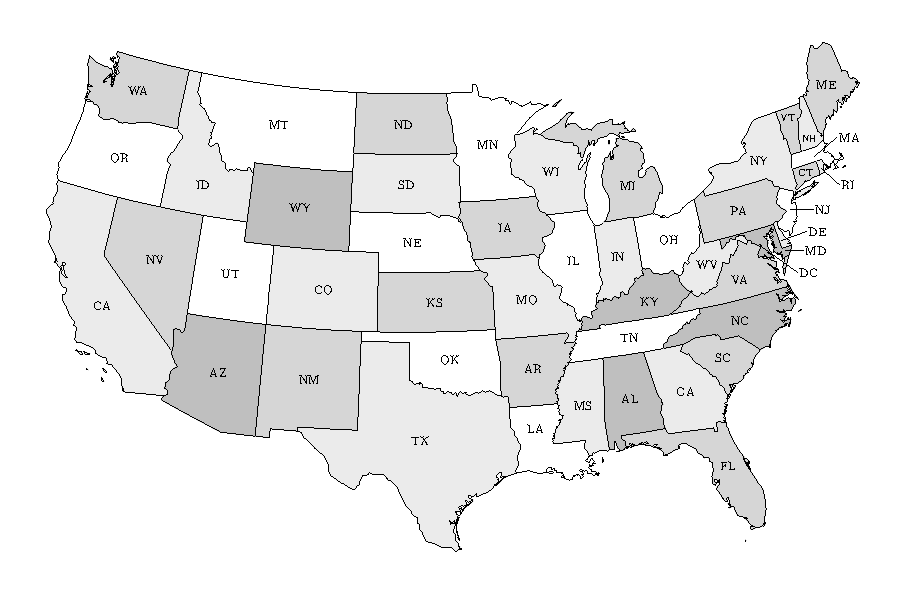
\includegraphics[scale=0.6,draft=false]{../../results/us_migration/us_migration_map_state_names.pdf}
	\vspace*{-0.5cm}
	\caption{US map with state boundaries and state abbreviations}
	\label{fig:notes_us_map} 
\end{figure}







\section{Word count}

The word count of this dissertation is \input{texcount.txt}\unskip, obtained using \TeX \hspace*{-0.15cm} count by running
%
\begin{center}
	\texttt{texcount -relaxed -inc -0 -sum=1,1,1,0,0,0,0 <dissertation.tex>\,}.
\end{center}
%
%The final dissertation should be no longer than 7,500 words, this usually equates to 25--30 pages. The word count may exclude any table of contents, all mathematical equations and symbols, diagrams, tables, bibliography and the texts of computer programs. However any preface, footnotes, and appendices must be included













